% This file is part of JTS-MM (https://github.com/paulotto/jts-mm).
% SPDX-FileCopyrightText: 2026 Paul-Otto Müller
% SPDX-License-Identifier: CC-BY-4.0

\section{Dimensioned drawings and FreeCAD recipe}\label{sec:drawings}
\subsection{How to build the parts in FreeCAD}\label{sec:freecad}
Every part is either a \emph{profile swept along a curve that follows the teeth} (bars, jaws, pads,
wires) or a \emph{conforming shell} (the flange of concept~1 and the plate of concept~3). The folder
\texttt{cad/} contains everything needed to place the profiles:
\begin{itemize}
\item \texttt{import\_reference\_geometry.FCMacro}: run it with the FCStd open. It creates
\begin{description}[style=nextline,leftmargin=2em]
\item[\texttt{REF\_curves}] B-spline sweep paths on the tooth surface (offset by \SI{0.05}{mm},
interdental notches closed with a \SI{2.5}{mm} rolling ball), the wire centrelines of concepts 3
and 4, and the arch centreline.
\item[\texttt{REF\_sections}] one sketch per station, placed in the section plane with
\textbf{sketch $x = n$} (positive buccal) and \textbf{sketch $y = h$} (from the lowest cusp tip,
positive toward the gum). The tooth outline is included as construction geometry. The
coordinates in the section drawings below can be typed in directly. (In FreeCAD the model's gum
side is $+z$, so the sketch appears upside down relative to the drawings.)
\item[\texttt{REF\_path\_starts}] one sketch at the start of every sweep path, same orientation,
origin on the path: draw the profile relative to the path there.
\end{description}
\item The same curves as DXF (one file each and \texttt{all\_reference\_geometry.dxf}) and CSV
($x,y,z,s$), and \texttt{stations.csv} with position, tangent and normal of every station.
\end{itemize}

\paragraph{Recipe.}
\begin{enumerate}
\item Open the FreeCAD file with the teeth model
(\texttt{parts/teeth\_attachment/teeth\_attachment.FCStd}), run the macro. Optionally import the concept
STL from \texttt{stl/} as a visual check; it sits on the teeth.
\item \textbf{Long parts} (lingual bar, labial bar, yoke): open the matching \texttt{START\_} sketch,
draw the profile from the section drawing \emph{relative to the path} (e.g.\ lingual bar: rectangle
$x\in[-2.0,\,0]$, $y\in[-1.4,\,+1.4]$), then \emph{Part $\rightarrow$ Sweep}: profile = sketch,
path = the \texttt{REF\_} curve, \emph{Solid} on, \emph{Frenet} off. This was tested on the
lingual bar path.
\item \textbf{Short parts on one tooth} (jaws, pads, loop module, TPU insert, rests): draw the
profile in \texttt{SEC\_M1\_mid\_R} and \emph{Pad} it symmetrically by its length along the arch
(from the plan view and parameter table). Over \SIrange{7}{9}{mm} the molar face is straight to
about \SI{0.1}{mm}; the resin reline takes up the rest.
\item \textbf{Wires}: sweep a circle of the wire diameter along \texttt{REF\_c4\_wire\_mounted} or
\texttt{REF\_c3\_adams\_*} (for visualisation and clearance checks only; the real wire is bent on
the model).
\item \textbf{Conforming shells} (concepts 1 and 3): start from \texttt{stl/c1\_printed.stl} /
\texttt{stl/c3\_rigid.stl}, or offset a blocked-out tooth model (Meshmixer, Blender) by the wall
thickness; a parametric sweep cannot follow the crown shape.
\item Mirror left/right with \emph{Part $\rightarrow$ Mirror} about the plane through
\texttt{REF\_ref\_centreline\_h6p0} at $s=0$ only if the subject's arch is symmetric enough; the
reference curves exist for both sides.
\item Fuse, add retention holes for the resin (Ø\SI{1.2}{mm}, \SI{3}{mm} pitch) and the
\SI{0.1}{mm} relief on non-contacting faces, export STL.
\end{enumerate}

\subsection{Reference dimensions of the dental arch}
\begin{figure}[H]\centering
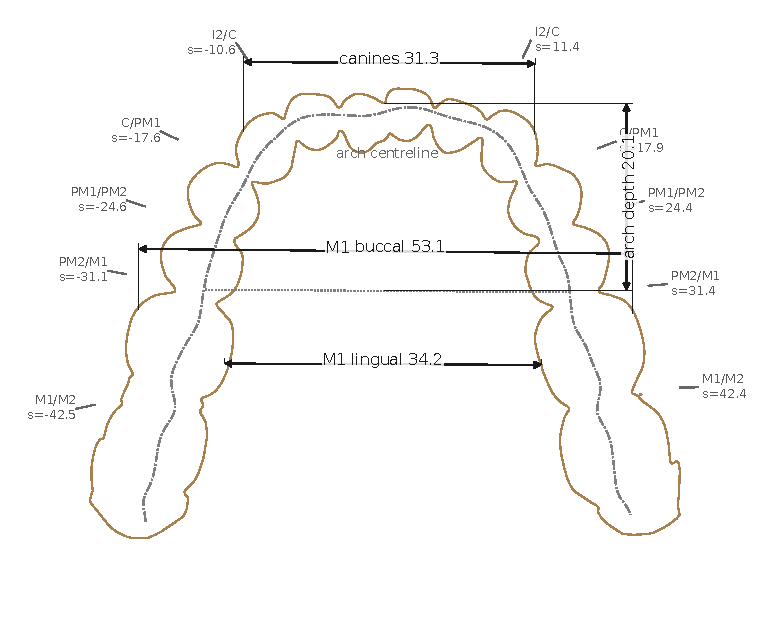
\includegraphics[width=0.72\textwidth]{drw_ref_plan}
\caption{Occlusal plan of \texttt{Teeth\_02} (section at $h=6.5$), $X=x-x_\text{midline}$, anterior
at the top. Stations $s$ are arc lengths along the centreline; all drawings refer to them.}
\label{fig:drw_ref}
\end{figure}
\begin{table}[H]\centering\small
\caption{Measured on \texttt{Teeth\_02} (\texttt{s09\_drawings.py}).}\label{tab:refdims}
\begin{tabular}{l S[table-format=2.1]}
\toprule dimension & {mm}\\ \midrule
\inputrows{generated/ref_dims.tex}
\bottomrule
\end{tabular}
\end{table}

\newcommand{\paramtable}[2]{%
\begin{table}[H]\centering\small\caption{#2}\label{tab:params_#1}
\begin{tabularx}{\textwidth}{X l l}\toprule parameter & key in \texttt{params.py} & value [mm, deg]\\ \midrule
\inputrows{generated/params_#1.tex}
\bottomrule\end{tabularx}\end{table}}

\subsection{Common parts}
\begin{figure}[H]\centering
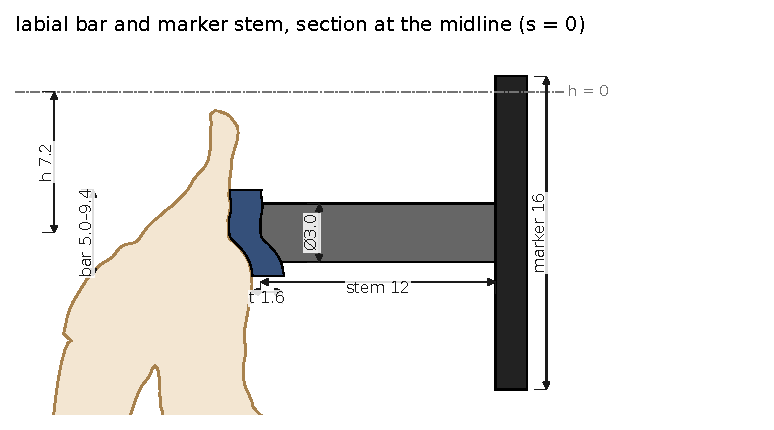
\includegraphics[width=0.8\textwidth]{drw_common_marker}
\caption{Labial bar and marker stem at the midline. The labial bar is the same in all concepts;
sweep its profile along \texttt{REF\_path\_labial\_h7p2} over $s=\pm16.5$.}
\label{fig:drw_common}
\end{figure}
\paramtable{common}{Common parameters.}

\subsection{Concept 1: snap shell}
\begin{figure}[H]\centering
\begin{subfigure}[b]{0.48\textwidth}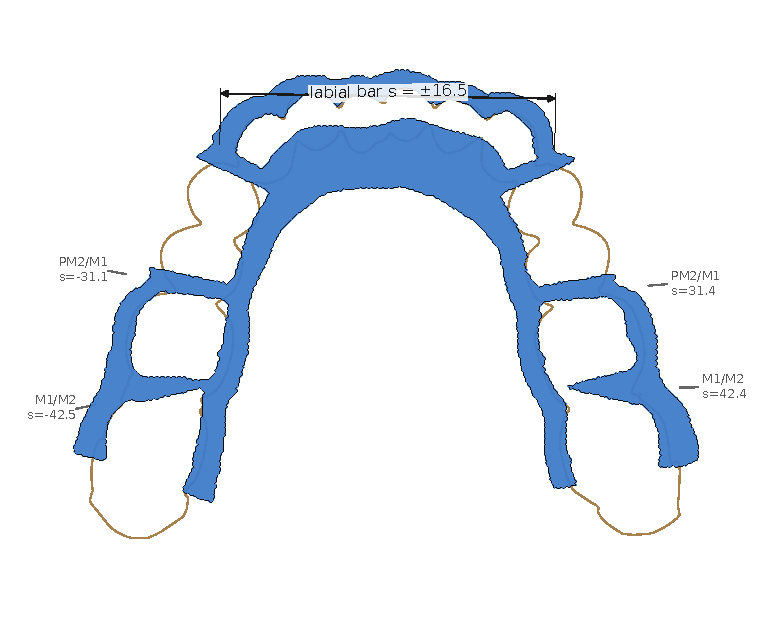
\includegraphics[width=\linewidth]{drw_c1_plan}\caption{plan}\end{subfigure}\hfill
\begin{subfigure}[b]{0.48\textwidth}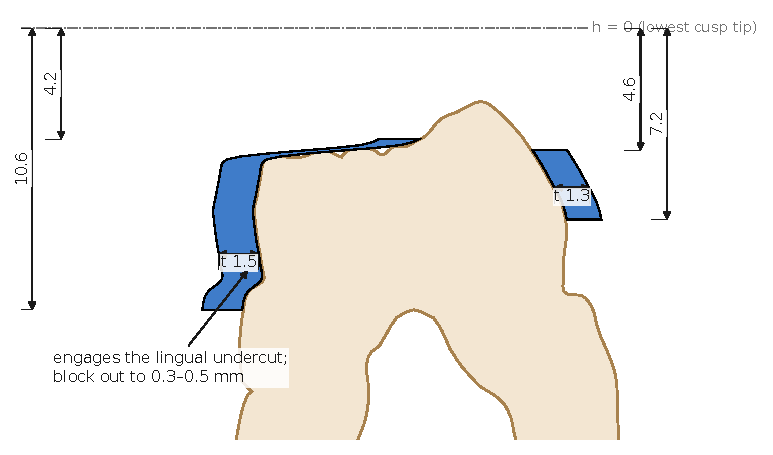
\includegraphics[width=\linewidth]{drw_c1_section}\caption{section at the right M1}\end{subfigure}
\caption{Concept 1. Build the shell from the STL or by offsetting (see recipe); the section gives the thicknesses and extents.}\label{fig:drw_c1}
\end{figure}
\paramtable{c1}{Concept 1 parameters.}

\subsection{Concept 2: clothespin jaw}
\begin{figure}[H]\centering
\begin{subfigure}[b]{0.46\textwidth}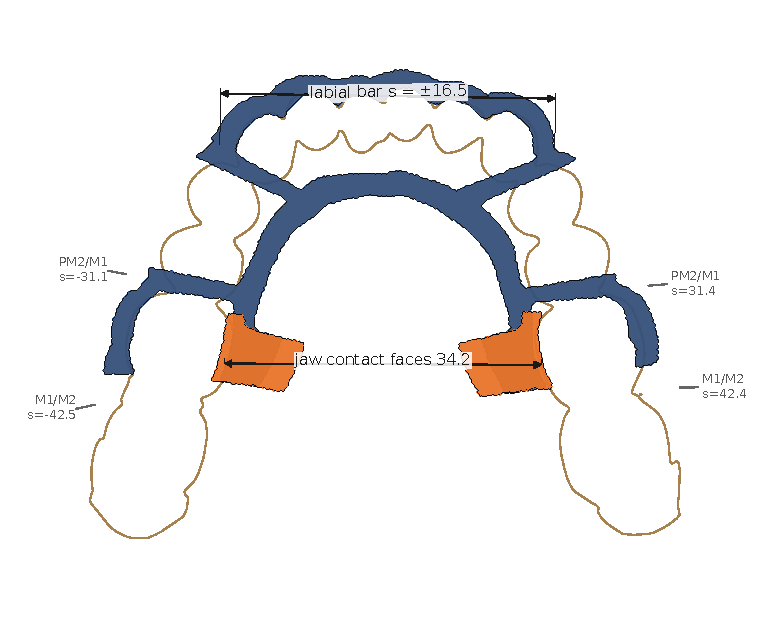
\includegraphics[width=\linewidth]{drw_c2_plan}\caption{plan}\end{subfigure}\hfill
\begin{subfigure}[b]{0.52\textwidth}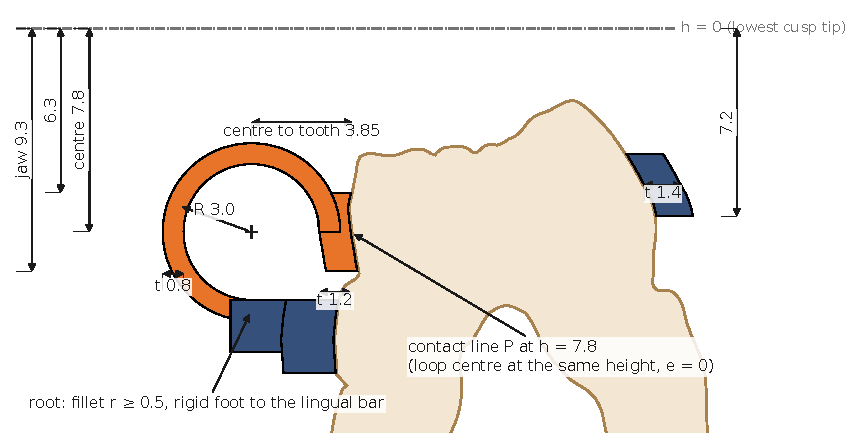
\includegraphics[width=\linewidth]{drw_c2_section}\caption{section at the right M1}\end{subfigure}\\[2mm]
\begin{subfigure}[b]{\textwidth}\centering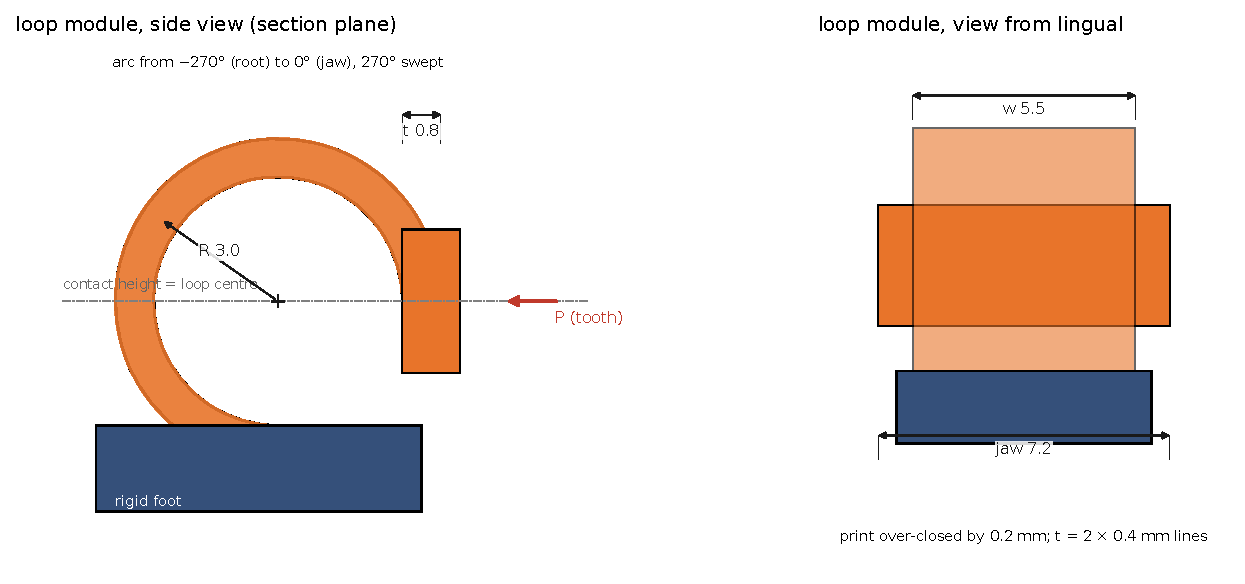
\includegraphics[width=0.9\linewidth]{drw_c2_loop}\caption{loop module (clip-in part)}\end{subfigure}
\caption{Concept 2. Lingual bar: sweep a \SI{2.0}{mm}$\times$\SI{2.8}{mm} rectangle along
\texttt{REF\_path\_lingual\_bar\_h11p8}. Buccal jaw, loop module and foot: pad from
\texttt{SEC\_M1\_mid\_R}. Loop sizing: \cref{sec:loop}.}\label{fig:drw_c2}
\end{figure}
\paramtable{c2}{Concept 2 parameters.}

\subsection{Concept 3: wire clasps}
\begin{figure}[H]\centering
\begin{subfigure}[b]{0.46\textwidth}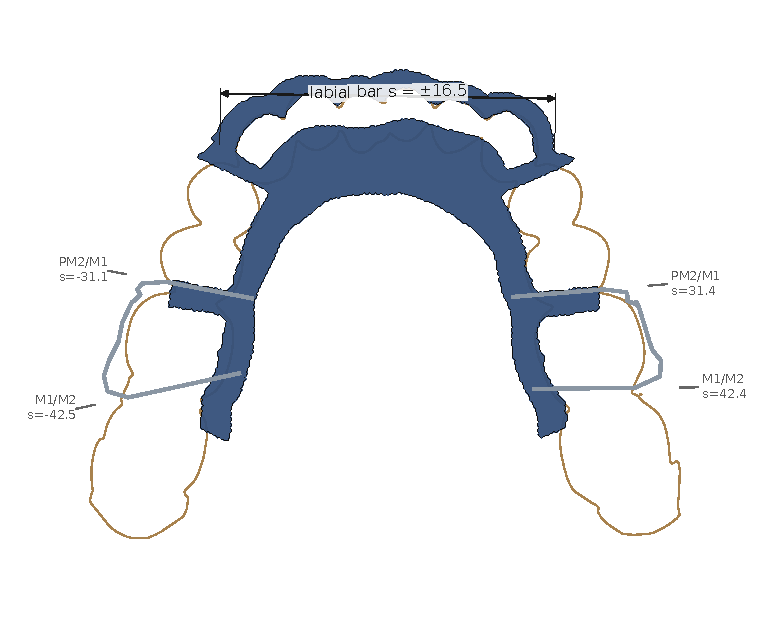
\includegraphics[width=\linewidth]{drw_c3_plan}\caption{plan}\end{subfigure}\hfill
\begin{subfigure}[b]{0.50\textwidth}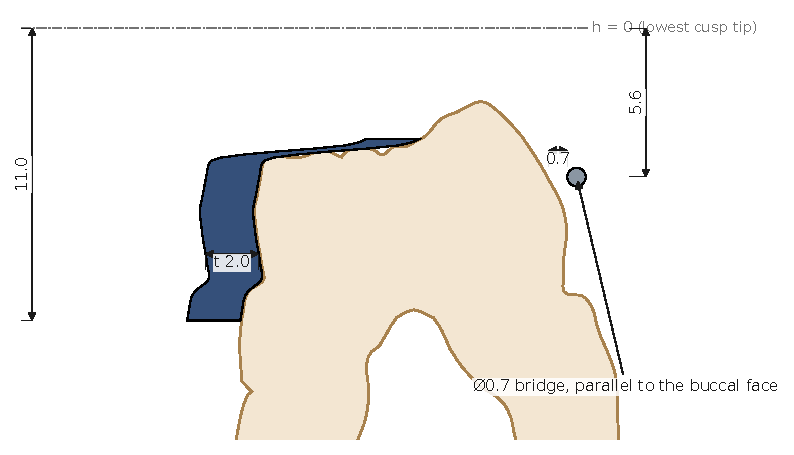
\includegraphics[width=\linewidth]{drw_c3_section}\caption{section at the right M1}\end{subfigure}\\[2mm]
\begin{subfigure}[b]{\textwidth}\centering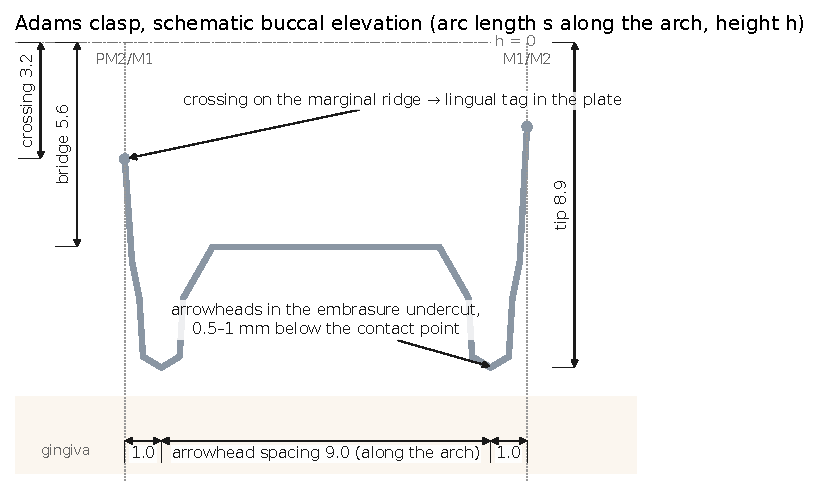
\includegraphics[width=0.8\linewidth]{drw_c3_adams}\caption{Adams clasp}\end{subfigure}
\caption{Concept 3. The plate is a conforming shell; the clasp is bent on the model following (c) and
\texttt{REF\_c3\_adams\_*}.}\label{fig:drw_c3}
\end{figure}
\paramtable{c3}{Concept 3 parameters.}

\subsection{Concept 4: spring arch}
\begin{figure}[H]\centering
\begin{subfigure}[b]{0.48\textwidth}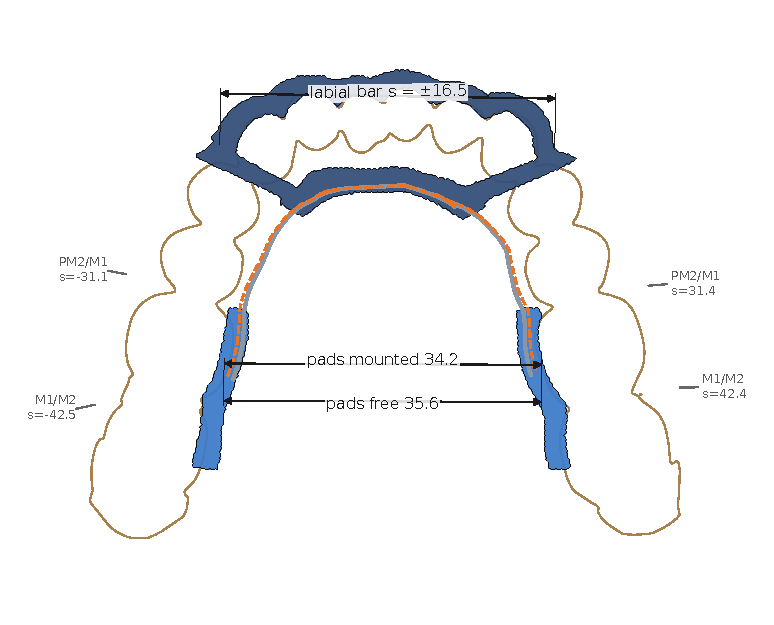
\includegraphics[width=\linewidth]{drw_c4_plan}\caption{plan: wire mounted (grey) and free (dashed)}\end{subfigure}\hfill
\begin{subfigure}[b]{0.48\textwidth}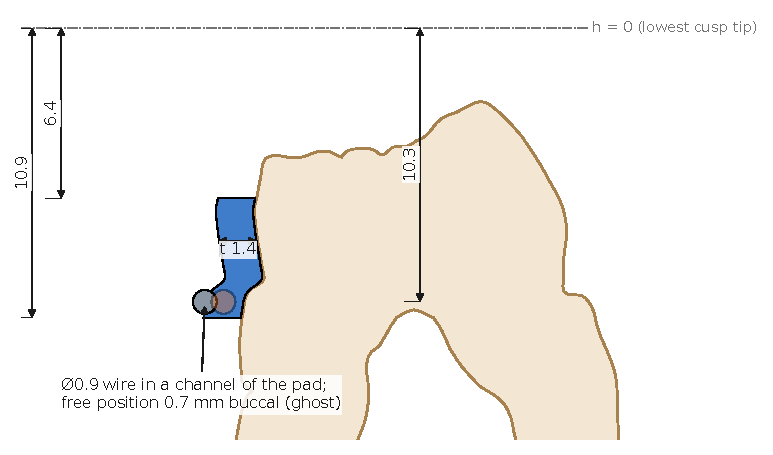
\includegraphics[width=\linewidth]{drw_c4_section}\caption{section at the right M1}\end{subfigure}
\caption{Concept 4. Bend the wire to \texttt{REF\_c4\_wire\_free} (the mounted shape spread by
\SI{0.7}{mm} per side); pads: pad the section profile over the M1 and M2 station ranges.}\label{fig:drw_c4}
\end{figure}
\paramtable{c4}{Concept 4 parameters.}

\subsection{Concept 5: rigid clamp with TPU liner}
\begin{figure}[H]\centering
\begin{subfigure}[b]{0.46\textwidth}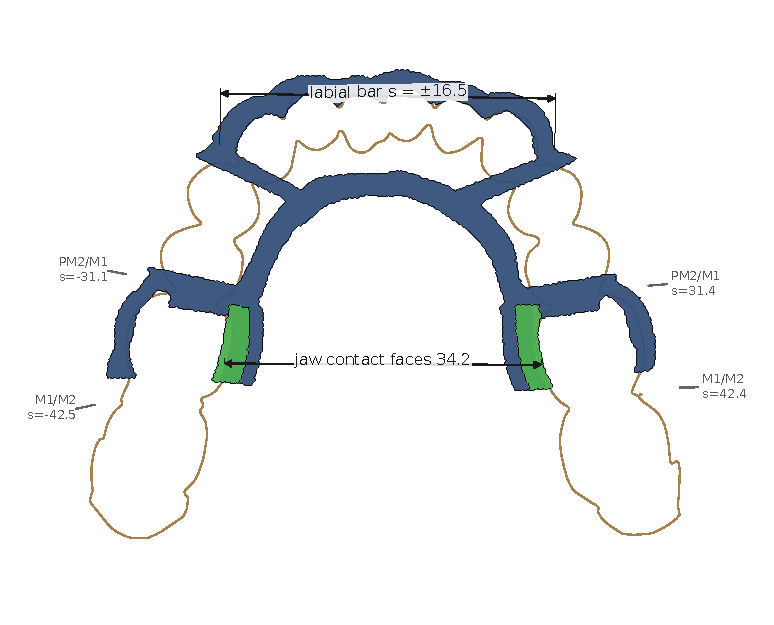
\includegraphics[width=\linewidth]{drw_c5_plan}\caption{plan}\end{subfigure}\hfill
\begin{subfigure}[b]{0.50\textwidth}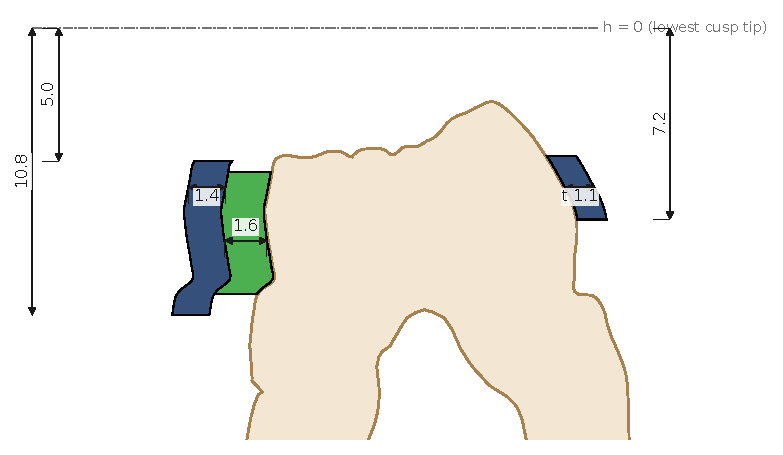
\includegraphics[width=\linewidth]{drw_c5_section}\caption{section at the right M1}\end{subfigure}\\[2mm]
\begin{subfigure}[b]{\textwidth}\centering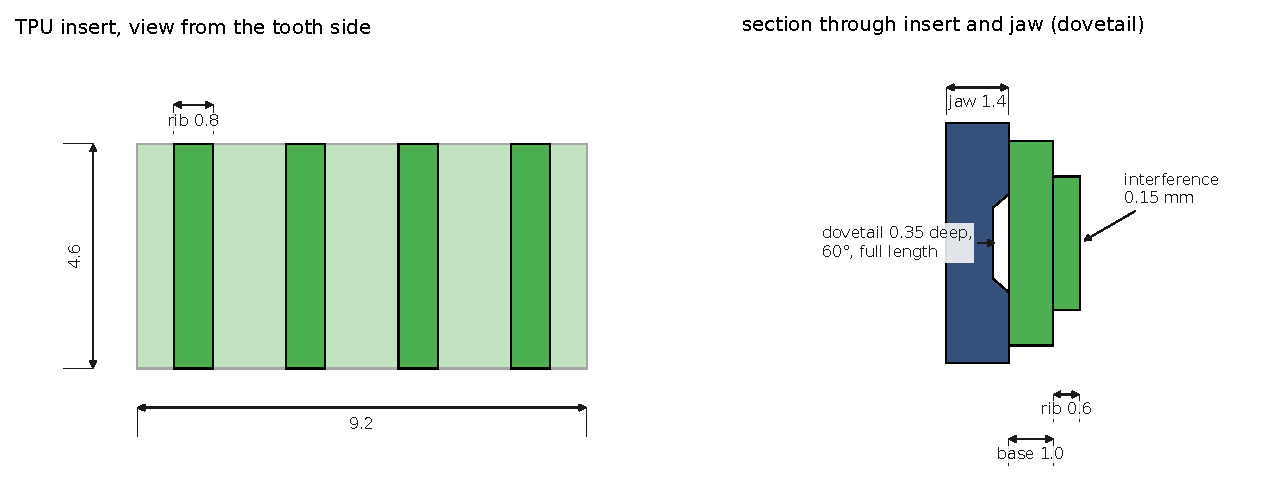
\includegraphics[width=0.85\linewidth]{drw_c5_insert}\caption{TPU insert and dovetail}\end{subfigure}
\caption{Concept 5. The TPU insert slides into a dovetail in the rigid jaw; interference is set by
the insert thickness.}\label{fig:drw_c5}
\end{figure}
\paramtable{c5}{Concept 5 parameters.}
